\documentclass[12pt, a4paper]{article}
\usepackage{enumitem}
\usepackage[left=2cm, right=2cm, top=2cm, bottom=2cm]{geometry}
\usepackage{float}
\usepackage{graphicx}
\usepackage[colorlinks, urlcolor=blue]{hyperref}
\usepackage{xeCJK}

\renewcommand\arraystretch{1.1}
\setCJKmainfont{新細明體}

\title{
  Network Administration/System Administration\\
  (NTU CSIE, Spring 2024)\\
  Homework \#3
}
\author{\Large B12902110 呂承諺}
\date{}

\begin{document}
  \maketitle

  \section{Initial partition}
  \paragraph{Steps}
  \begin{enumerate}
    \item Run \verb|fdisk /dev/vda|.
    \item Run the following commands inside \verb|fdisk|:
    \begin{footnotesize}
      \begin{verbatim}
Command (m for help): g
Created a new GPT disklabel (GUID: C55CEE8B-500E-4F53-BD71-CD40DA22FBE1).

Command (m for help): n
Partition number (1-128, default 1):
First sector (2048-2097118, default 2048):
Last sector, +/-sectors or +/-size{K,M,G,T,P} (2048-2097118, default 2095103): +1M

Created a new partition 1 of type 'Linux filesystem' and of size 1 MiB.

Command (m for help): t
Selected partition 1
Partition type or alias (type L to list all): 4
Changed type of partition 'Linux filesystem' to 'BIOS boot'.

Command (m for help): n
Partition number (2-128, default 2):
First sector (4096-2097118, default 4096):
Last sector, +/-sectors or +/-size{K,M,G,T,P} (4096-2097118, default 2095103): +100M

Created a new partition 2 of type 'Linux filesystem' and of size 100 MiB.

Command (m for help): n
Partition number (3-128, default 3):
First sector (208896-2097118, default 208896):
Last sector, +/-sectors or +/-size{K,M,G,T,P} (208896-2097118, default 2095103):

Created a new partition 3 of type 'Linux filesystem' and of size 921 MiB.

Command (m for help): t
Partition number (1-3, default 3): 3
Partition type or alias (type L to list all): 44

Changed type of partition 'Linux filesystem' to 'Linux LVM'.

Command (m for help): w\end{verbatim}
    \end{footnotesize}
  \end{enumerate}
  \paragraph{Result}
   Below is the output of \verb|fdisk -l /dev/vda|:\\[1.5ex]
   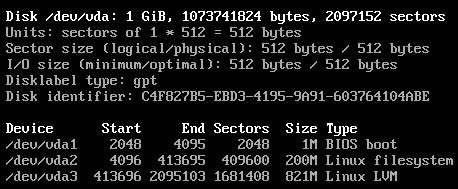
\includegraphics[width=0.7\textwidth]{1_result.png}
  \paragraph{References}
  \begin{itemize}
    \item \verb|fdisk| partition types
  \end{itemize}

  \section{RAID Setup}
  \paragraph{Steps}
    Run the following commands:
    \begin{verbatim}
mdadm --create /dev/md127 --level 10 --name data --raid-devices 4 \
  /dev/vdc /dev/vdd /dev/vde /dev/vdf
mdadm --create /dev/md126 --level 0 --name linux --raid-devices 2 \
  /dev/vda3 /dev/vdb\end{verbatim}
  \paragraph{Result}
  Below is the output of \verb|cat /proc/mdstat|:\\[1.5ex]
  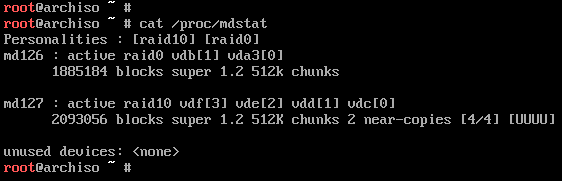
\includegraphics[width=0.7\textwidth]{2_result.png}
  \paragraph{References}
  \begin{itemize}
    \item \verb|mdadm --create --help|
  \end{itemize}

  \section{Disk encryption}
  \paragraph{Steps}
  \begin{enumerate}
    \item Encrypt \verb|/dev/vda2| and map it to \verb|/dev/mapper/cryptboot|:
    \begin{verbatim}
cryptsetup luksFormat --type luks1 /dev/vda2
cryptsetup open /dev/vda2 cryptboot\end{verbatim}
    \item Generate a random 256-bit key, and add it as a key of
    \verb|/dev/mapper/cryptboot|:
    \begin{verbatim}
dd if=/dev/random of=b12902110.key bs=256 count=1
cryptsetup luksAddKey /dev/vda2 b12902110.key\end{verbatim}
    \item Encrypt \verb|/dev/md/linux| and map it to \verb|/dev/mapper/cryptroot|:
    \begin{verbatim}
cryptsetup luksFormat --type luks2 /dev/md/linux b12902110.key
cryptsetup open /dev/md/linux cryptroot\end{verbatim}
    \item Encrypt \verb|/dev/md/data| and map it to \verb|/dev/mapper/cryptdata|:
     \begin{verbatim}
cryptsetup lukfFormat --type luks2 /dev/md/data b12902110.key
cryptsetup open /dev/md/data cryptdata\end{verbatim}
  \end{enumerate}
  \paragraph{Result}
  Below is the output of \verb|lsblk -f| and \verb|cryptsetup status|:\\[1.5ex]
  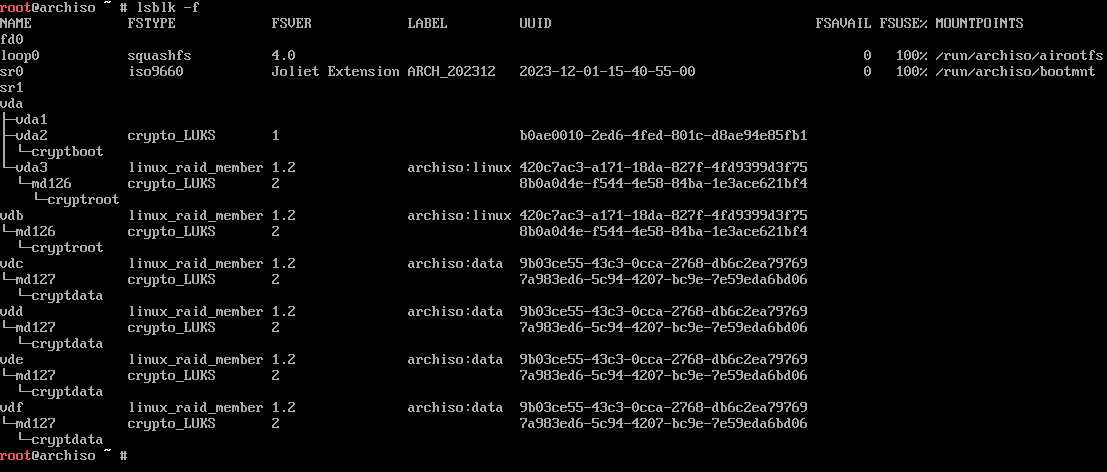
\includegraphics[width=\textwidth]{3_result_lsblk.png}\\[1.5ex]
  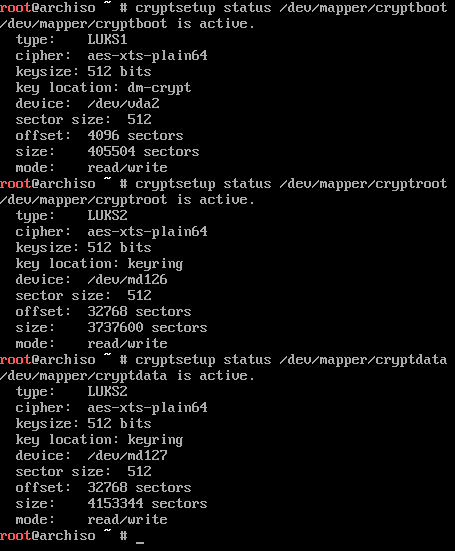
\includegraphics[width=0.5\textwidth]{3_result_cryptsetup_status.png}

  \paragraph{References}
  \begin{itemize}
    \item \href{https://wiki.archlinux.org/title/dm-crypt/Device_encryption}{dm-crypt/Device encryption - ArchWiki}
    \item \href{https://en.wikipedia.org/wiki/Linux_Unified_Key_Setup}{Linux Unified Key Setup - Wikipedia}
    \item \verb|man dd|
    \item \href{https://unix.stackexchange.com/questions/148062/mdadm-raid-doesnt-mount}{mdadm raid doesn't mount - Unix \& Linux Stack Exchange}
    \item \href{https://unix.stackexchange.com/questions/260533/how-to-determine-what-encryption-is-being-used-a-luks-partition}{How to determine what encryption is being used a LUKS partition? - Unix \& Linux Stack Exchange}
    \item \verb|man lsblk|
  \end{itemize}

  \section{LVM Setup}
  \paragraph{Steps}
  Run the following commands:
    \begin{verbatim}
pvcreate /dev/mapper/cryptroot
vgcreate linux /dev/mapper/cryptroot
lvcreate --size 256M --name home linux
lvcreate --extents 100%FREE --name root linux cryptdata\end{verbatim}
  \paragraph{Result}
  Below is the output of \verb|pvs|, \verb|vgs|, \verb|lvs|, and
  \verb|fdisk -l|:\\[1.5ex]
  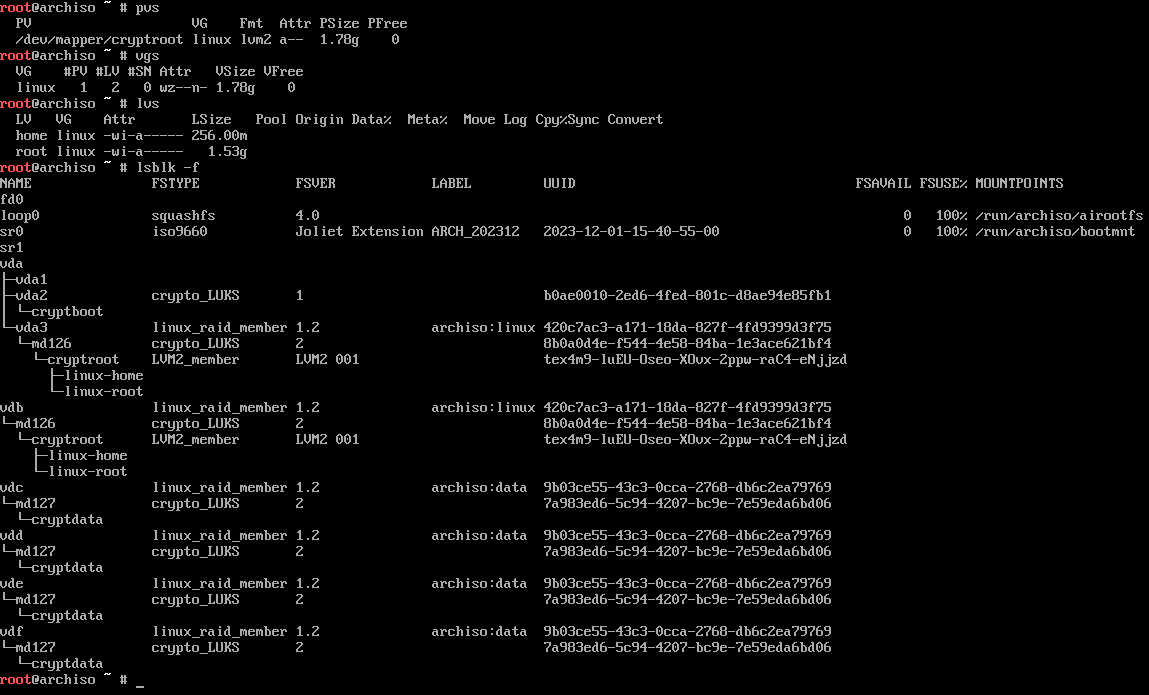
\includegraphics[width=\textwidth]{4_result.png}
  \paragraph{References}
  \begin{itemize}
    \item \verb|man pvcreate|, \verb|man vgcreate| and \verb|man lvcreate|
    \item \href{https://hackmd.io/@aoaaceai/rJ0xXBnhT#/8/3}{Section ``LVM usage" of ``Partition lab 2024 - HackMD"}
  \end{itemize}

  \section{Formatting}
  \paragraph{Steps}
  Run the following commands:
    \begin{verbatim}
mkfs.ext4 /dev/linux/home
mkfs.ext4 /dev/linux/root
mkfs.xfs /dev/mapper/cryptdata
mkfs.ext2 /dev/mapper/cryptbooot\end{verbatim}
  \paragraph{Result}
  Below is the output of \verb|fdisk -l| after formatting:\\[1.5ex]
  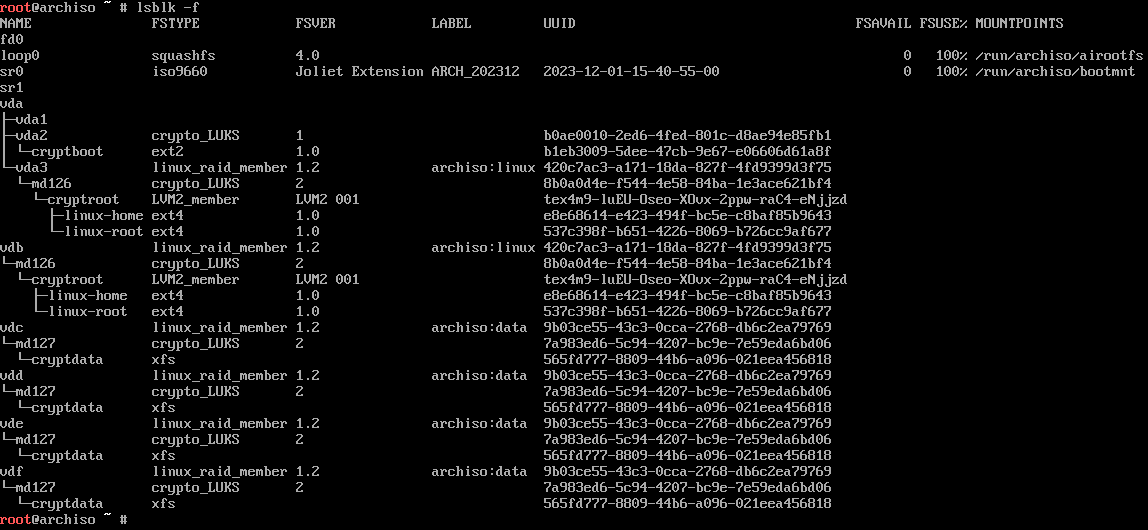
\includegraphics[width=\textwidth]{5_result.png}

  \section{Mounting}
  \paragraph{Steps}
  Run the following commands:
    \begin{verbatim}
mount /dev/linux/root /mnt
mount /dev/linux/home /mnt/home --mkdir
mount /dev/mapper/cryptboot /mnt/boot --mkdir
mount /dev/mapper/cryptdata /mnt/data --mkdir\end{verbatim}
  \paragraph{Result}
  Below is the output of \verb|mount| and \verb|ls -alh /mnt|:\\[1.5ex]
  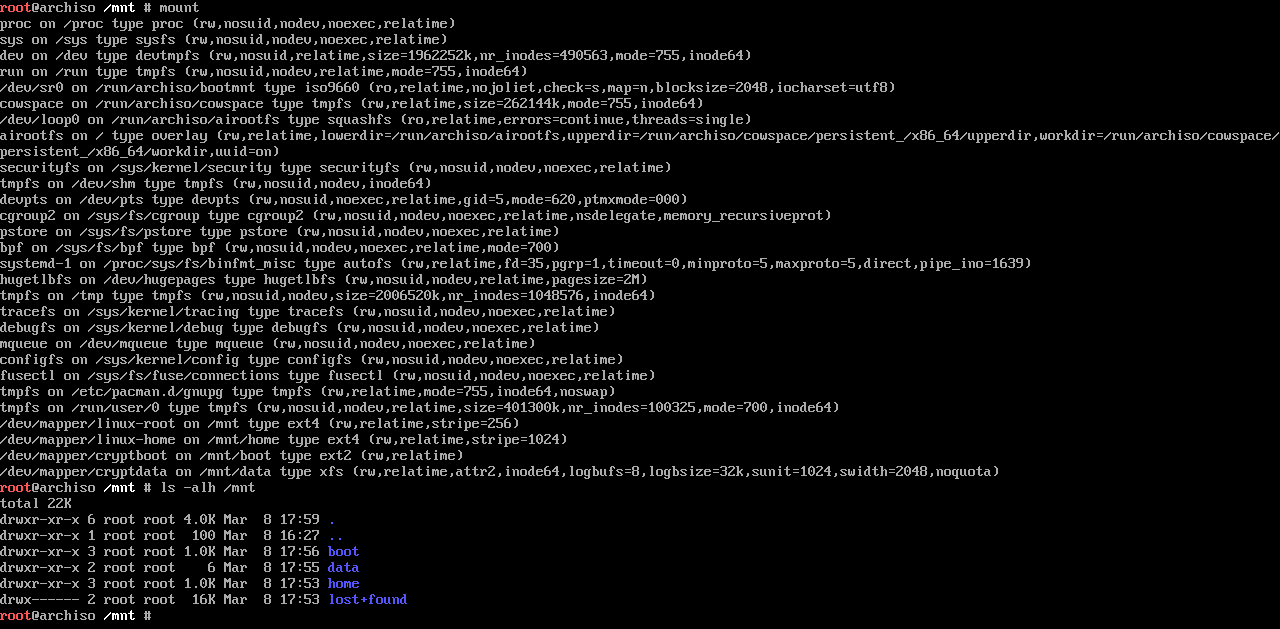
\includegraphics[width=\textwidth]{6_result.png}

  \section{Arch Installation}
  \paragraph{Steps}
  \begin{itemize}
    \item Run \verb|pacman -Sy --needed archlinux-keyring| to update
    \verb|archlinux-keyring| to the latest version 20240208-1. Otherwise we
    would get ``signature is unknown trust" errors.
    \item Follow \href{https://wiki.archlinux.org/title/installation_guide#Installation}{ArchWiki's installation guide}
    and run the following commands:
    \begin{verbatim}
pacstrap -K /mnt base linux

genfstab -U /mnt >> /mnt/etc/fstab

arch-chroot /mnt

pacman -Syu
pacman -S mdadm lvm2 nano man

ln -s /usr/share/zoneinfo/Asia/Taipei /etc/localtime
hwclock --systohc

# Edit /etc/locale.gen and uncomment en_US.UTF-8.
locale-gen
echo "LANG=en_US.UTF-8" > /etc/locale.conf

# Edit /etc/hostname and change hostname to new-arch-b12902110.

passwd\end{verbatim}
    \item Move key generated by step 3 to \verb|/etc/cryptsetup-keys.d|.
    \item Edit \verb|/etc/mkinitcpio.conf| and add \verb|encrypt|, \verb|lvm2|,
    \verb|mdadm_udev| to \verb|HOOKS|.\\
    Also add \verb|/etc/cryptsetup-keys.d/b12902110.key| to \verb|FILES|.
    \item Run \verb|mkinitcpio -p linux|.
    \item Add the following lines to  \verb|/etc/crypttab|:
    \begin{footnotesize}
      \begin{verbatim}
# UUID of /dev/vda2
cryptboot UUID=b0ae0010-2ed6-4fed-801c-d8ae94e85fb1 /etc/cryptsetup-keys.d/b12902110.key
# UUID of /dev/md/data
cryptdata UUID=7a983ed6-5c94-4207-bc9e-7e59eda6bd06 /etc/cryptsetup-keys.d/b12902110.key\end{verbatim}
  \end{footnotesize}
    \item Run \verb|pacman -S grub| to Install GRUB.
    \item Edit the following lines in \verb|/etc/default/grub|:
    \begin{footnotesize}
      \begin{verbatim}
GRUB_CMDLINE_LINUX="root=/dev/linux/root \
cryptdevice=UUID=8b0a0d4e-f544-4e58-84ba-1e3ace621bf4:cryptroot \
cryptkey=rootfs:/etc/cryptsetup-keys.d/b12902110.key"

GRUB_ENABLE_CRYPTODISK=y\end{verbatim}
    \end{footnotesize}
    \item Run the following commands:
    \begin{verbatim}
grub-install /dev/vda
grub-mkconfig -o /boot/grub/grub.cfg\end{verbatim}
  \end{itemize}

  \paragraph{Result}
  After rebooting and logging in, we see that all volumes have been correctly
  mounted.
  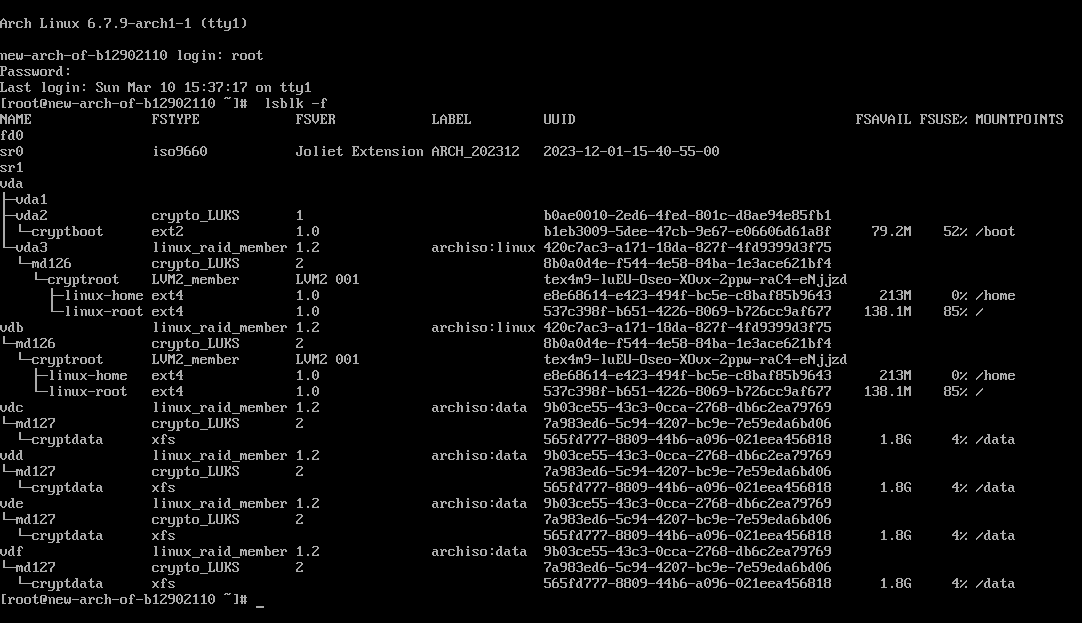
\includegraphics[width=\textwidth]{7_result.png}


  \paragraph{References}
  \begin{itemize}
    \item \href{https://wiki.archlinux.org/title/installation_guide#Installation}{Installation guide - ArchWiki (Installation)}
    \item \href{https://man.archlinux.org/man/pacstrap.8}{pacstrap(8) — Arch manual pages}
    \item \verb|man genfstab|, \verb|man arch-chroot|, \verb|man hwclock|
    \item \href{https://wiki.archlinux.org/title/Change_root}{chroot - ArchWiki}
    \item \href{https://man.archlinux.org/man/locale.conf.5}{locale.conf(5) — Arch manual pages}
  \end{itemize}
  Fixing package signature issue:
  \begin{itemize}
    \item \href{https://bbs.archlinux.org/viewtopic.php?id=289421}{[Resolved] Can't import and use PGP keys / Pacman \& Package Upgrade Issues / Arch Linux Forums}
    \item \href{https://wiki.archlinux.org/title/Pacman/Package_signing#Signature_is_unknown_trust}{pacman/Package signing - ArchWiki (Signature is unknown trust)}
  \end{itemize}
  \verb|mkinitcpio|:
  \begin{itemize}
    \item \href{https://wiki.archlinux.org/title/Mkinitcpio}{mkinitcpio - ArchWiki}
    \item \href{https://docs.kernel.org/filesystems/ramfs-rootfs-initramfs.html#what-is-rootfs}{Ramfs, rootfs and initramfs — The Linux Kernel  documentation}
    \item \href{https://wiki.archlinux.org/title/RAID#Configure_mkinitcpio}{RAID - ArchWiki (Configure mkinitcpio
    )}
  \end{itemize}
  Encryption:
  \begin{itemize}
    \item \href{https://wiki.archlinux.org/title/dm-crypt/System_configuration#Unlocking_in_late_userspace}{dm-crypt/System configuration - ArchWiki (Unlocking in late userspace)}
    \item \href{https://man.archlinux.org/man/crypttab.5.en}{crypttab(5) — Arch manual pages}
    \item \href{https://wiki.archlinux.org/title/dm-crypt/System_configuration#mkinitcpio}{dm-crypt/System configuration - ArchWiki (mkinitcpio)}
    \item \href{https://wiki.archlinux.org/title/Kernel_parameters}{Kernel parameters - ArchWiki}
    \item \href{https://wiki.archlinux.org/title/Arch_boot_process}{Arch boot process - ArchWiki}
    \item \href{https://wiki.archlinux.org/title/GRUB#Encrypted_/boot}{GRUB - ArchWiki (Encrypted /boot)}
    \item \href{https://wiki.archlinux.org/title/Dm-crypt/Device_encryption#With_a_keyfile_embedded_in_the_initramfs}{dm-crypt/Device encryption - ArchWiki (With a keyfile embedded in the initramfs
    )}
    \item \href{https://wiki.archlinux.org/title/Dm-crypt/Encrypting_an_entire_system#Encrypted_boot_partition_(GRUB)}{dm-crypt/Encrypting an entire system - ArchWiki (Encrypted boot partition (GRUB)}
  \end{itemize}
  GRUB and booting:
  \begin{itemize}
    \item \href{https://en.wikipedia.org/wiki/Master_boot_record}{Master boot record - Wikipedia}
    \item \href{https://en.wikipedia.org/wiki/Boot_sector}{Boot sector - Wikipedia}
    \item \href{https://en.wikipedia.org/wiki/GNU_GRUB}{GNU GRUB - Wikipedia}
    \item \href{https://www.gnu.org/software/grub/manual/grub/html_node/BIOS-installation.html#BIOS-installation}{GNU GRUB Manual 2.12: BIOS installation}
    \item \href{https://www.gnu.org/software/grub/manual/grub/html_node/Simple-configuration.html#Simple-configuration}{GNU GRUB Manual 2.12: Simple configuration}
    \item \href{https://man.archlinux.org/man/grub-install.8.en}{grub-install(8) — Arch manual pages}
  \end{itemize}
  Others:
  \begin{itemize}
    \item \href{https://wiki.archlinux.org/title/Install_Arch_Linux_on_LVM}{Install Arch Linux on LVM - ArchWiki}
    \item \href{https://bbs.archlinux.org/viewtopic.php?id=243391}{[SOLVED] LVM on LUKS Installation - emergency shell on boot / Installation / Arch Linux Forums}
    \item \href{https://www.shellhacks.com/mount-lvm-partition-in-rescue-mode/}{Mount LVM Partition in Rescue Mode - ShellHacks}
  \end{itemize}

  \section{Trivia}
  \begin{enumerate}[label=(\alph*)]
    \item The partition table. That is Master Boot Record (MBR) or GUID Partition Table (GPT).
    \item By default, 5\% of the filesystem blocks will be reserved for the super-user.
      We can see this by running \texttt{tunefs -l DEVICE | grep Reserved}.

      References:
      \begin{itemize}
        \item \href{https://askubuntu.com/questions/249387/df-h-used-space-avail-free-space-is-less-than-the-total-size-of-home}{disk usage - df -h - Used space + Avail Free space is less than the Total size of /home - Ask Ubuntu}
        \item \href{https://wiki.archlinux.org/title/ext4#Reserved_blocks}{Ext4 - ArchWiki (Reserved blocks)}
      \end{itemize}

    \item
      \begin{itemize}
        \item \textbf{FUSE:} A software interface that allows non-privileged users
          to create their own file systems without needing to modify the kernel
          code directly. The developer uses the \verb|libfuse| library to write
          a handler program that handle file I/Os.
        \item \textbf{Advantages:} Can be written in any popular programming
          language. Easier to debug.
        \item \textbf{Disadvantage:} May be slower.
        \item \textbf{Examples:} GlusterFS, GmailFS.
      \end{itemize}

      References:
      \begin{itemize}
        \item \href{https://en.wikipedia.org/wiki/Filesystem_in_Userspace}{Filesystem in Userspace - Wikipedia}
        \item \href{https://www.quora.com/What-is-the-advantage-of-FUSE-file-system-in-user-space}{What is the advantage of FUSE (file system in user space)? - Quora}
        \item \href{https://superuser.com/questions/312375/what-makes-a-fuse-file-system-different-than-a-kernel-file-system}{linux - What makes a fuse file system different than a kernel file system? - Super User}
      \end{itemize}

    \item MBR vs. GPT:
      \begin{table}[H]
        \centering
        \begin{tabular}{|c|c|c|}
        \hline
        & \textbf{MBR} & \textbf{GPT}\\\hline
        Meaning & Master Boot Record & GUID Partition Table \\\hline
        Maximum partitions & 4 primary, or 3 primary and  1 extended & 128 \\\hline
        Maximum disk sectors & $2^{32}$ sectors & $2^{64}$ sectors \\\hline
        \end{tabular}
      \end{table}

      References:
      \begin{itemize}
        \item \href{https://en.wikipedia.org/wiki/Master_boot_record}{Master boot record - Wikipedia}
        \item \href{https://en.wikipedia.org/wiki/GUID_Partition_Table#History}{GUID Partition Table - Wikipedia}
        \item \href{https://learn.microsoft.com/en-us/windows-hardware/manufacture/desktop/configure-uefigpt-based-hard-drive-partitions}{UEFI/GPT-based hard drive partitions | Microsoft Learn}
      \end{itemize}

    \item \verb|mount -t ntfs3 DEVICE MOUNTPOINT|

      References:
      \begin{itemize}
        \item \href{https://en.wikipedia.org/wiki/Comparison_of_file_systems}{Comparison of file systems - Wikipedia}
        \item \href{https://en.wikipedia.org/wiki/ExFAT}{exFAT - Wikipedia}
        \item \href{https://en.wikipedia.org/wiki/NTFS}{NTFS - Wikipedia}
        \item \href{https://wiki.archlinux.org/title/NTFS}{NTFS - ArchWiki}
        \item \href{https://docs.kernel.org/filesystems/ntfs3.html}{NTFS3 — The Linux Kernel  documentation}
      \end{itemize}

    \item 1 GB (gigabyte) = $10^9$ bytes. 1 GiB (gibibyte) = $1024^3$ bytes = $1073741824$ bytes.
      \verb|ls -h| uses powers of 1024 by default.

      References:
      \begin{itemize}
        \item \href{https://en.wikipedia.org/wiki/Gigabyte}{Gigabyte - Wikipedia}
        \item \verb|man ls|
      \end{itemize}

    \item Assuming 4 disks. 1st is fastest, 4th is slowest.
      \begin{table}[H]
        \centering
        \begin{tabular}{|c|c|c|c|}
        \hline
        & Redundancy (Max. disks that we can lose) & Read speed & Write speed \\\hline
        RAID 0 & 0 & 1st & 1st \\\hline
        RAID 10 & 2 (only if 1 in every RAID 1) & 2nd & 4th \\\hline
        RAID 5 & 1 & 3rd & 2st \\\hline
        RAID 6 & 2 & 3rd & 3rd \\\hline
        \end{tabular}
      \end{table}

      References:
      \begin{itemize}
        \item \href{https://en.wikipedia.org/wiki/Standard_RAID_levels}{Standard RAID levels - Wikipedia}
        \item \href{https://en.wikipedia.org/wiki/Nested_RAID_levels#RAID_10}{Nested RAID levels - Wikipedia}
      \end{itemize}

    \item Maybe because encryption overhead is the bottleneck, that is, the
      slowest process of all processes.
  \end{enumerate}
\end{document}
